\title{The Graph Hessian}

Everybody knows about the graph Laplacian, but can we define the Hessian
operator on a graph?  Let us see.

\section{Recall of algebraic graph calculus}

Consider a directed graph~$G=(V,E)$ with~$n$ vertices and~$m$ edges.

\newcommand{\R}{\mathbf{R}}
\newcommand{\Z}{\mathbf{Z}}

Functions~$f:V\to\R$ are called~\emph{scalar fields}
and they are elements of~$\R^n$.

Functions~$X:E\to\R$ are called~\emph{vector fields} and they are elements
of~$\R^m$.  For an intuition, you may think that the values of~$X$ on the
edges around a vertex~$p\in V$ are the components of the vector~$X_p$.


The~\emph{signed incidence matrix}~$B$ has~$m$ rows and~$n$ columns, encoding
the directed edges with~$\pm 1$.  More precisely, if~$e=(i,j)\in E$ this
means that~$B_{ei}=-1$, $B_{ej}=1$ and zero elsewhere.  The linear
operator~$B:\R^n\to\R^m$ transforms scalar fields into vector fields and is
called the~\emph{gradient}.  Given a scalar field~$f:V\to\R$, its gradient is
a vector field that at each edge~$e=(i,j)\in E$ takes the value~$f(j)-f(i)$.

The linear operator~$-B^\top:\R^m\to\R^n$ transforms vector fields into
scalar fields and is called the~\emph{divergence}.  Given a vector
field~$X:E\to\R$ its divergence is a scalar field that represents the
difference between the inflow and outflow at each vertex.

The~\emph{laplacian} is the divergence of the gradient~$L=-B^\top B$.  As
an~$n\times n$ matrix, it is symmetric and negative semidefinite.  As a
linear operator, it transforms scalar fields into scalar fields.  The
condition~$Lf=0$ for a scalar field~$f$ is an equilibrium condition:
the value of~$f$ at one vertex is equal to the average value on all its
neighbours.

These definitions are analogous to the corresponding constructions of vector
calculus in~$\R^2$ and~$\R^3$.  However, not all operations that we can do in
vector calculus are possible here.  For example, the pointwise product of a
scalar and a vector field is not well defined in the discrete case.  For that
we'll need to introduce a specific~\emph{centering
operator} defined by~$C=\frac12\left|B\right|$.

The centering operator~$C:\R^n\to\R^m$ transforms scalar fields into vector
fields, just like the gradient; but it takes the average instead of the
difference at each edge. Similarly, the operator~$C^\top$ takes vector fields
into scalar fields.

Thanks to the centering operator we can prove the discrete analogs of the
traditional product rules from vector calculus
\begin{equation}\label{eq:vectorcalculus}
	\nabla\left(fg\right)=f\nabla g+g\nabla f
	\qquad
	\qquad
	\mathrm{div}\left(fX\right)
	=f\mathrm{div}X+X\cdot\nabla f
\end{equation}

In the discrete case, to avoid algebraic confusion,
we will denote pointwise products in~$\R^d$
by~$\odot_d$.  Thus the pointwise product of two scalar fields~$f$ and~$g$ is
the scalar field~$f\odot_n g$.  We also define the product of a scalar
field~$f$ with a vector field~$X$ as the vector field~$Cf\odot_m X$, and the
dot product of two vector fields~$X$ and~$Y$ as the scalar
field~$C^\top\left(X\odot_m Y\right)$

We readily check the product rule for the discrete gradient:
\begin{equation}\label{eq:gradprod}
	B\left(f\odot_n g\right)=
	Cf\odot_m Bg + Bf\odot_m Cg
\end{equation}
and, with some more work, the product rule for the divergence
\begin{equation}\label{eq:divprod}
	-B^\top\left(Cf\odot_m X\right)
	=
	f\odot_n\left(-B^\top X\right)
	+C^\top\left(X\odot_m Bf\right)
\end{equation}
Notice that formulas~\eqref{eq:gradprod} and~\eqref{eq:divprod} may appear
complicated at first sight, but they are the exact translation of the
traditional product rules~\eqref{eq:vectorcalculus}.  You don't need to
remember these complicated formulas: you deduce them every time you need, by
writing the traditional product rule and adding centering operators until the
dimensions fit.

{\color{gray}
An interesting particular case of these computations is when~$G$ is the
one-dimensional path graph.  For example let~$V=\Z$ with edges joining
consecutive integers from low to high.  Now, if~$f:\Z\to\R$ is a discrete
function, the gradient~$Bf$ is the discrete derivative computed by forward
differences (which is defined at half-positions, that is, on the edges!).
The operator~$-B^\top$ is backwards finite differences, and composing both we
obtain the second derivative~$L f$ by the traditional three-point scheme:
\[
	Lf (i) = f(i-1) -2f(i)+f(i+1)
\]
Using the traditional (but confusing) notation for finite
differences~$\Delta_1 f(i)=f(i+1)-f(i)$, we can rewrite the
formula~\eqref{eq:gradprod} as
\[
	\Delta_1(fg)(i) =
	\tfrac{f(i)+f(i+1)}2\Delta_1 g(i) +
	\tfrac{g(i)+g(i+1)}2\Delta_1 f(i)
\]
which is the most natural form of the product rule for discrete derivatives
(exact, and with only two terms, unlike some horrendous monstrosities that
are often found in numerical analysis books).  Here we see that the centering
operator is necessary, but it arises in a natural way.
}

Finally, as a sanity check, we can verify the
product rule for the Laplacian:~$\Delta\left(fg\right)=f\Delta g+g\Delta
f+2\nabla f\cdot\nabla g$:
\[
	L\left(fg\right)=
	f\odot_n Lg
	+
	g\odot_n Lf
	+2C^\top\left(Bf\odot_m Bg\right)
\]
This follows directly by applying equations~\eqref{eq:gradprod}
and~\eqref{eq:divprod} one after the other.


\clearpage
\section{Numerical verification}

None of this would be any good if it wasn't easy to verify numerically.  Let
us check whether all these derivatives make sense for a 2D image.  I do these
experiments because the formulas that we'll find later for the Hessian will
be so scary that we'll need to verify them...

Let us consider a~$128\times128$ image with a Gaussian profile, together with
some of its derivatives


\begin{tabular}{cccccc}

\includegraphics{fgauss.png} &

\includegraphics{fgaussx.png} &

\includegraphics{fgaussy.png} &

\includegraphics{fgaussxx.png} &

\includegraphics{fgaussxy.png} &
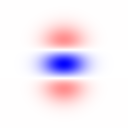
\includegraphics{fgaussyy.png} \\
$u$ & $u_x$ & $u_y$ & $u_{xx}$ & $u_{xy}$ & $u_{yy}$
\end{tabular}
%SCRIPT plambda zero:128x128 ":r 2 ^ -0.1 / exp" -o fgauss.npy
%SCRIPT palette {-,}1 nice fgauss.npy fgauss.png
%SCRIPT plambda fgauss.npy "x,x"|palette {-,}0.05 nice - fgaussx.png
%SCRIPT plambda fgauss.npy "x,y"|palette {-,}0.05 nice - fgaussy.png
%SCRIPT plambda fgauss.npy "x,xx"|palette {-,}0.005 nice - fgaussxx.png
%SCRIPT plambda fgauss.npy "x,xy"|palette {-,}0.005 nice - fgaussxy.png
%SCRIPT plambda fgauss.npy "x,yy"|palette {-,}0.005 nice - fgaussyy.png
%SCRIPT plambda fgauss.npy "x,g"|viewflow 0.05 - fgaussg.png
%SCRIPT plambda fgauss.npy "x,n"|palette {-,}0.08 nice - fgaussgn.png
%SCRIPT plambda fgauss.npy "x,l"|palette {-,}0.005 nice - fgaussl.png
%SCRIPT plambda fgauss.npy "x,xx x,yy * x,xy 2 ^ -"|palette {-,}0.00004 nice - fgaussd.png
%SCRIPT plambda fgauss.npy "x,xx x,x 2 ^ * x,yy x,y 2 ^ * x,xy x,x x,y * * -2 * + +"|palette {-,}0.000005 nice - fgaussc.png
%SCRIPT plambda fgauss.npy "x,g dup vnorm /"|plambda "x,d -1 *"|palette {-,}1 nice - fgaussk.png

\bigskip

\begin{tabular}{cccccc}

\includegraphics{fgaussgn.png} &

\includegraphics{fgaussg.png} &

\includegraphics{fgaussl.png} &

\includegraphics{fgaussd.png} &

\includegraphics{fgaussc.png} &

\includegraphics{fgaussk.png} \\
$\left\|\nabla u\right\|$ &
$\mathrm{vec}\left(\nabla u\right)$ &
$\Delta u$ &
$\mathrm{det}H u$ &
$\mathrm{canny}(u)$ &
$\mathrm{curv}(u)$
\end{tabular}

For reference, these images have been produced using the following shell
script
 \begin{verbatim}
plambda zero:128x128 ":r 2 ^ -0.1 / exp" -o fgauss.npy
palette {-,}1 nice fgauss.npy fgauss.png
plambda fgauss.npy "x,x"  | palette {-,}0.05  nice - fgaussx.png
plambda fgauss.npy "x,y"  | palette {-,}0.05  nice - fgaussy.png
plambda fgauss.npy "x,xx" | palette {-,}0.005 nice - fgaussxx.png
plambda fgauss.npy "x,xy" | palette {-,}0.005 nice - fgaussxy.png
plambda fgauss.npy "x,yy" | palette {-,}0.005 nice - fgaussyy.png
\end{verbatim}%x


% vim:set tw=77 filetype=tex spell spelllang=en:
